\begin{enumerate}[label={$\arabic*.$}]
	\item Scheibe: $n(R,z)=n_0\cdot\left(e^{-\frac{|z|}{h_\text{thin}}}+\num{0.02}\cdot e^{-\frac{|z|}{h_\text{thick}}}\right)\cdot e^{-\frac{R}{h_R}}$\\
		$h_R=\SI{3.5}{k\ps}$\\
		$h_\text{thin}=\SI{325}{\ps},\ h_\text{thick}=\SI{1.5}{k\ps}$
	\item Bulge:\\
		Skalenhöhe ($\propto e^{-\frac{|z|}{h_z}}$): $h_z=\SI{0.4}{k\ps}$\\
		$I(R)=I_e\cdot e^{-\num{7.669}\cdot\left(\left(\frac{R}{R_e}\right)^\frac{1}{4}-1\right)}$ de Vancouleurs-Profil\\
		$R_e$: Effektivradius, innerhalb dessen die Hälfte der Leuchtkraft emittiert wird.
	\item Stellarer Halo:\\
		$n(r)\propto r^{-\num{3.5}}$ Dichteverteilung\\
		mit de Vancouleurs-Profil: $r_e\approx \SI{3}{k\ps}$
	\item DM Halo: \\
		quasi-isothermal: $n(r)\propto\frac{1}{a^2+r^2},a=\SI{12}{k\ps} \begin{pmatrix} a & \text{definiert} \\ n & \text{bei $r=0$}\end{pmatrix}$\\
		Navarro-Frenk-White Modell: $n_{NFM}\propto\frac{1}{\frac{r}{r_s}\left(1+\frac{r}{r_s}\right)^2}$ $r_s\approx\SI{12}{k\ps}$
\end{enumerate}
\subsection{Die Rotationskurve der Galaxis}
\begin{itemize}
	\item Motivitation: Bestimmung der Rotationsgeschwindigkeit $V=V(R)$ as Funktion des Abstands $R$ von galaktischem Zentrum (GC)
		\begin{figure}[H]
			\begin{tikzpicture}
				\coordinate (a) at (0,0);
				\coordinate (b) at (0,-3);
				\coordinate (c) at (2,-1.5);
				\coordinate (d) at (0,-1.5);
				\node[name=v0] at (2,0){$V_0$};
				\draw[->, shorten <= 4pt,shorten >= 2pt] (a)circle(3pt)--(v0);
				\draw (a)--(b)node[midway,left]{$R_0$};
				\draw[->] (b)--(c)node[below right]{$\vec{r}$}node[midway,below right]{$R$};
				\draw[dashed] (d)--(c);
				\draw (a)--(c);
				\pic[draw,"$\theta$",angle eccentricity=1.5] {angle = c--b--a};
				\pic[draw,"$l$",angle eccentricity=1.5] {angle=b--a--c};
			\end{tikzpicture}
		\end{figure}
	\item (kreisförmige) Bewegung in der galaktischen Ebene: $\vec{r}=R\begin{pmatrix}\sin(\theta) \\ \cos(\theta)\end{pmatrix}, \vec{V}=\dot{\vec{r}}=V(R)\cdot\begin{pmatrix} \cos(\theta) \\ -\sin(\theta) \end{pmatrix}$
	\item Mit Hilfe der Abbildung: $\vec{r}=\begin{pmatrix} D\cdot\sin(l) \\ R_0-D\cdot\cos(l) \end{pmatrix}$
		\begin{itemize}
			\item $\sin(\theta)=\frac{D}{R}\sin(l)$\\
				$\cos(\theta)=\frac{R_0}{R}-\frac{D}{R}\cos(l)$\\
				mit $\vec{V}_\odot\approx \vec{V}_\text{LSR}=\begin{pmatrix} V_0 \\ 0 \end{pmatrix}$\\
					$\Delta\vec{V}=\vec{V}-\vec{V}_\odot=\begin{pmatrix} V\frac{R_0}{R}-V\frac{D}{R}\cos(l)-V_0 \\ -V\frac{D}{R}\sin(l)\end{pmatrix}= \begin{pmatrix} R_0-(\Omega-\Omega_0)-\Omega\cdot D\cdot\cos(l) \\ -\Omega D \sin(l) \end{pmatrix}$ mit $\Omega(R)=\frac{V(R)}{R}$ der Winkelgeschwinditkeit $\Omega_0=\frac{V_0}{R_0}$
		\end{itemize}
	\item Komponenten der Relativbewegung zwischen Sonne und Objekten ergibt sich durch Projektion von $\vec{V}:$
		\begin{align*}
			v_r&=\Delta \vec{V}\cdot\begin{pmatrix}\sin(l)\\-\cos(l)\end{pmatrix}=(\Omega-\Omega_0)\cdot R_0\cdot\sin(l) \quad \text{Radialgeschwindigkeit}\\
				v_t&=\Delta \vec{V}\cdot\begin{pmatrix}\cos(l)\\ \sin(l)\end{pmatrix}=(\Omega-\Omega_0)\cdot R_0\cdot\cos(l)-\Omega\cdot D\quad\text{Tangentialgeschwindigkeit}
		\end{align*}
		Messung von $l$ und $v_r$ (Dopplereffekt, siehe 2.8.2) möglich über Eigenbewegung $\mu=\frac{v_t}{D}$ (siehe 2.8.2) erhält man $\Omega$ und $D$
	\item $R=\sqrt{R_0^2+D^2-2R_0D\cos(l)}$
	\item \underline{Problem}: Nicht möglich bei großen $D$ wegen Extinktion in der galaktischen Scheibe ($A_v\sim\SI{28}{\mag}$)
	\item Für kleine $D<<R_0$, lineare Näherung:
		\begin{equation*}
			(\Omega-\Omega_0)\approx\left(\frac{d\Omega}{dR}\right)|_{R_0}\cdot(R-R_0)+\cdots
		\end{equation*}
		\begin{align*}
			\Rightarrow v_r&= (R-R_0)\frac{d\Omega}{dR}|_{R_0}\cdot R_0\sin(l)\\
			&=(R-R_0)\frac{d}{dR}\left(\frac{V}{R}\right)|_{R_0}\cdot\sin(l)\\
			&\approx\left(\left(\frac{dV}{dR}\right)_{R_0}-\frac{V_0}{R_0}\right)\cdot\sin(l)(R-R_0)\\
			&\text{und } v_t=\left(\left(\frac{dV}{dR}\right)|_{R_0}-\frac{V_0}{R_0}\right)\cdot(R-R_0)\cos(l)-\Omega_0\cdot D
		\end{align*}
		Für $(R-R_0)<<R_0 \ \Rightarrow \ R_0-R\approx D\cos(l)$\\
		\begin{equation*}
			\Rightarrow v_r=AD\sin(l),\ v_r=AD\cos(2l)+B\cdot D
		\end{equation*}
		mit den Oortschen Koordinaten:
		\begin{align*}
			A&:=-\frac{1}{2}\left[\left(\frac{dV}{dR}\right)_{R_0}-\frac{V_0}{R_0}\right]\\
			B&:=-\frac{1}{2}\left[\left(\frac{dV}{dR}\right)_{R_0}+\frac{V_0}{R_0}\right]\\
			&\Rightarrow \Omega_0=\frac{V_0}{R_0}=A-B,\quad \left(\frac{dV}{dR}\right)_{R_0}=-(A+B)
		\end{align*}
		\begin{figure}[H]
			\begin{multicols}{2}
				\begin{figure}[H]
					\centering
					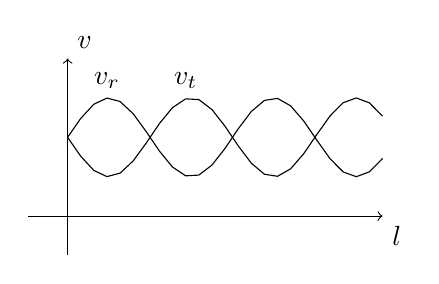
\begin{tikzpicture}
						\draw[->] (-0.5,0)--(4,0)node[below right]{$l$};
						\draw[->] (0,-0.5)--(0,2)node[above right]{$v$};
						\draw[domain=0:4,step=1000] plot(\x,{0.5*sin(540*\x/3.14156)+1});
						\draw[domain=0:4,step=1000] plot(\x,{-0.5*sin(540*\x/3.14156)+1});
						\node[above] at (0.5,1.5){$v_r$};
						\node[above] at (1.5,1.5){$v_t$};
					\end{tikzpicture}
				\end{figure}\columnbreak
				Messung ergibt:
				\begin{align*}
					A&=(\num{14.8}\pm\num{0.8})\si{\frac{\km}{\s}\frac{1}{k\ps}}\\
					B&=(-\num{12.4}\pm\num{0.6})\si{\frac{\km}{\s}\frac{1}{k\ps}}
				\end{align*}
			\end{multicols}
		\end{figure}
	\item Bestimmung von $V(R)$ für $R<R_0$:
		\begin{figure}[H]
			\begin{multicols}{2}
				\begin{figure}[H]
					\centering
					\begin{tikzpicture}
						\node[name=o,shape=circle,draw] at (0,0){};
						\draw (o)--(0,-4)node[name=gc,below]{GC};
						\draw (o)--(4,-5)coordinate(b);
						\pic[draw,"$l$",angle eccentricity=1.5] {angle=gc--o--b};
						\foreach \x in {1,...,5}{
							\draw[fill=white,pattern=north west lines] (0.8*\x,-\x)circle(0.3 cm)coordinate(x\x);
							\node[above right] at (0.8*\x+0.1,-\x+0.1){\x};
						};
						\draw (gc)--(x3)node[midway,below right]{$R_{min}$};
					\end{tikzpicture}
				\end{figure}\columnbreak
				\begin{figure}[H]
					\centering
					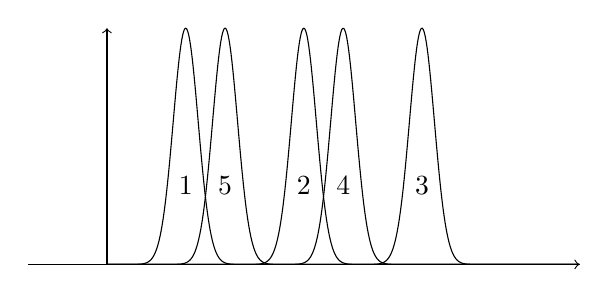
\begin{tikzpicture}
						\draw[->] (-1,0)--(6,0);
						\draw[->] (0,0)--(0,3);
						\foreach \y in {1,1.5,2.5,3,4}{
							\draw[domain=0:6,samples=500] plot(\x,{3*exp(-20*(\x-\y)^2)});
						}
						\node at (1,1){1};
						\node at (1.5,1){5};
						\node at (2.5,1){2};
						\node at (3,1){4};
						\node at (4,1){3};
					\end{tikzpicture}
				\end{figure}
			\end{multicols}
		\end{figure}
		\begin{itemize}
			\item Messung von $v_r$ mit Hilfe der $\SI{21}{\cm}$ Emissionslinie von neutralem Wasserstoff (galaktische Scheibe transparent für Radiowellen) mit  Hilfe des Doppler-Effekts
		\end{itemize}
	\item Unter der Annahme, dass sich das Gas der Galaxis auf Kreisbahnen um das GC bewegt, ist zu erwarten, dass für die Wolke im Tangentialpunkt (Wolke 3 im Bild) die gesamte Geschwindigkeit auf $v_r$ projeziert wird und sie daher die größte Radialgeschwinditkeit aufweist:
		\begin{align*}
			D&=R_0\cos(l), R_\text{min}=R_0\sin(l) \text{ und } \\
			V_{r,max}&=(\Omega(R_{min}-\Omega_0)R_0\sin(l)=V(R_{min})-V_0\\
			\Rightarrow V(R)&=\frac{R}{R_0}+V_0+V_{r,max}|_{\sin(l)=\frac{R}{R_0}}
		\end{align*}
		$A\neq 0\Rightarrow$ Galaxis rotiert nicht starr.
	\item Bestimmung von $V(R)$ für $R>R_0$: $v_r$ Messung an Objekten deren Entfernung $D_{max}$ bestimmen kann, z.B. Cepheiden
\end{itemize}
\underline{Resultat:}\\
\begin{figure}[H]
	\begin{tikzpicture}
		\draw[->] (-1,0)--(5,0);
		\draw[->] (0,0)--(0,3);
		\draw[domain=0:5,samples=100] plot(\x,{20*\x*exp(-5*\x)+2-2*exp(-\x)});
	\end{tikzpicture}
\end{figure}
\begin{itemize}
	\item Die Rotationskurve fällt nach außen hin ab, trotz einer Stern- und Gasdichte, die exponentiell abfällt:
		\begin{equation*}
			n(R,z)\approx n_0e^{-\frac{|z|}{h_z}}e^{-\frac{R}{h_z}} \text{ mit } h_z\approx\SI{0.3}{k\ps},\ h_R\approx\SI{3.5}{k\ps}
		\end{equation*}
	\item wenn es nur sichtbare Materie gäbe, würde Ian + Kepler gelten: $V(R)\sim R^{-\frac{1}{2}}$
	\item aber man erhält $V(R)\sim cnst.\ \Rightarrow M(R)\sim R$\\
		$\Rightarrow$ "`dunkle Materie"' (?)
\end{itemize}
